\section{Tutorial}

\begin{frame}
  \heading{Lets step into odeint}
  \tableofcontents[currentsection] 
\end{frame}


\begin{frame}[fragile]

\heading{Example -- Pendulum}

\vspace{2ex}

\begin{columns}[T]
  \begin{column}{0.35\textwidth}
    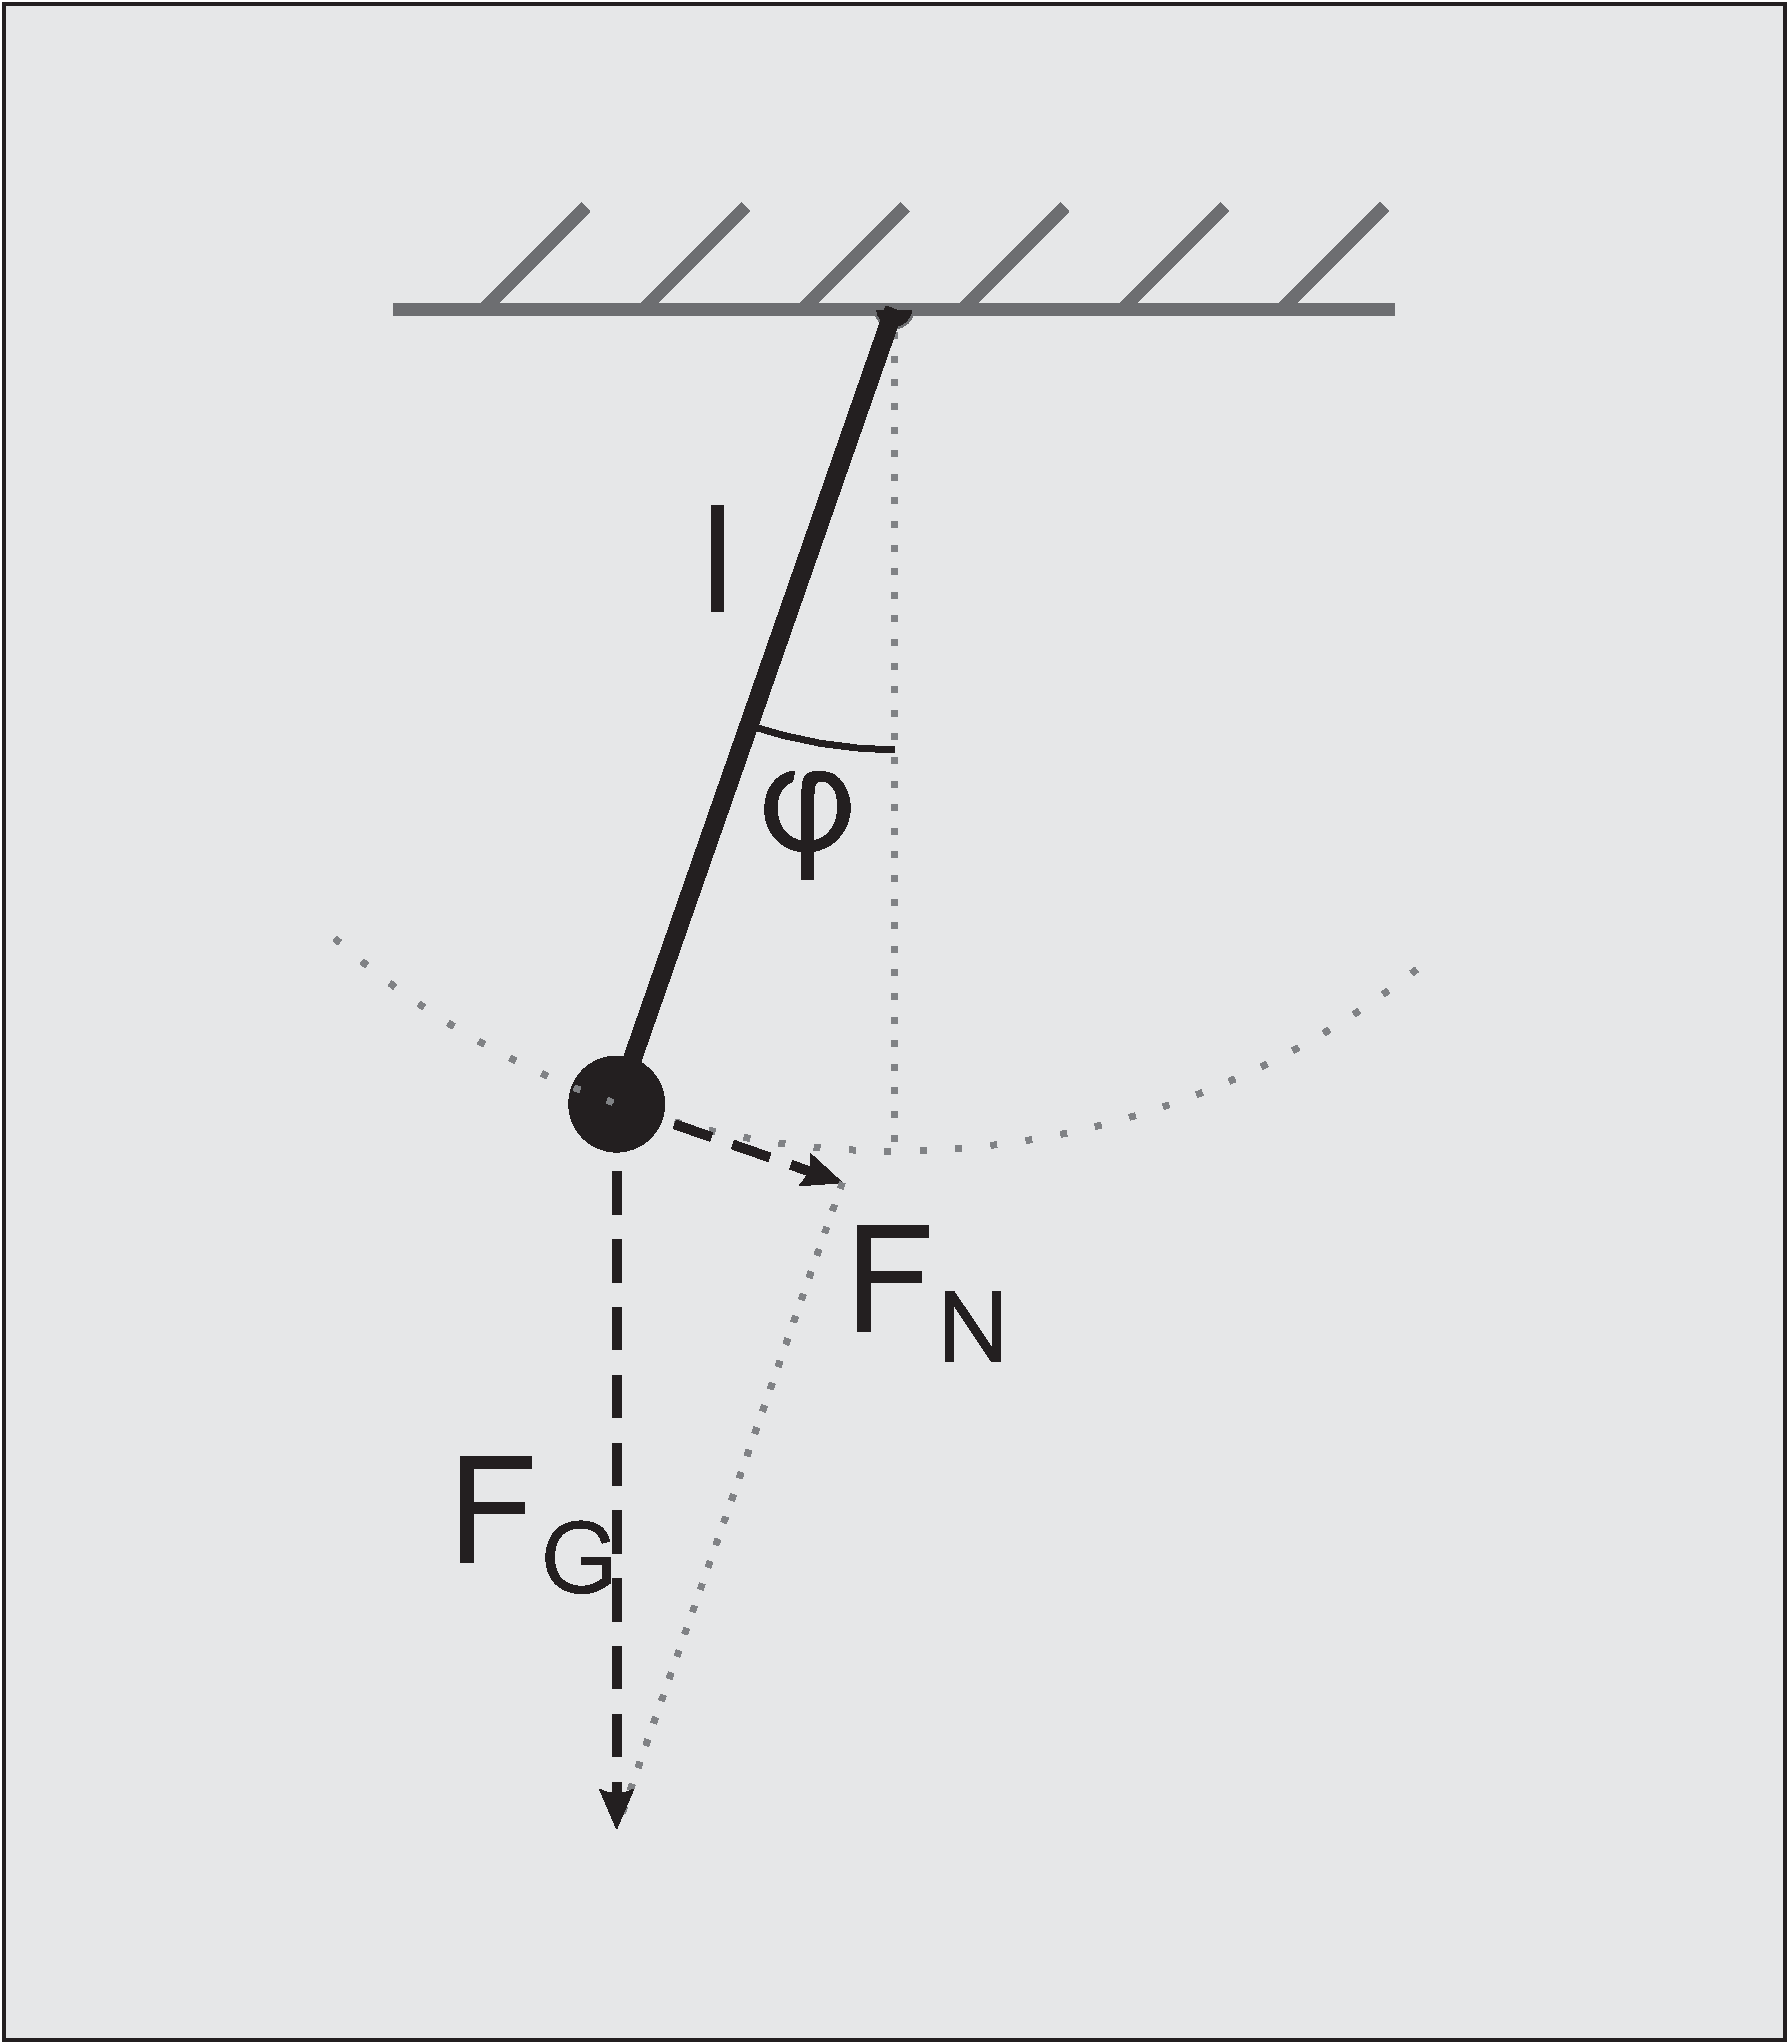
\includegraphics[draft=false,width=1.0\textwidth]{pendulum.pdf}

   \vspace{4ex}
  \end{column}

  \begin{column}{0.65\textwidth}
 \only<1>{
 Newtons law: $m a = F$

 \vspace{2ex}

 Acceleration:  $a = l \ddot{\varphi}$

 \vspace{2ex}

 Force: $F=F_N = - m g \sin \varphi$

 \vspace{4ex}

 $\Longrightarrow$ {\bf ODE for $\varphi$}

 $$\ddot{\varphi} = - g / l \sin \varphi = -\omega_0^2 \sin \varphi$$
 }

 \only<2>
 {

 $$\ddot{\varphi} = - \omega_0^2 \sin \varphi $$

 Small angle: $\sin \varphi \approx \varphi$

 \vspace{2ex}

 Harmonic oscillator $\ddot{\varphi} = - \omega_0^2 \varphi$

 \vspace{2ex}

 Analytic solution: $\varphi = A \cos \omega_0 t + B \sin \omega_0 t$

 \vspace{2ex}

 Determine $A$ and $B$ from initial condition\rem{:

 \centerline{$\varphi(t=0) = \varphi_0 \,\, \text{,} \quad \dot{\varphi}(t=0) = \dot{\varphi}_0$}

 \centerline{$B=\varphi_0 \,\, \text{,} \quad A=\dot{\varphi}_0 / \omega$}}

 }

 \only<3>{

 Full equation: $\ddot{\varphi} = -\omega_0^2 \sin \varphi $

 \vspace{2ex}

 Pendulum with friction and external driving:

 $$\ddot{\varphi} = -\omega_0^2 \sin \varphi - \mu \dot{\varphi} + \varepsilon \sin \omega_E t $$

 \vspace{2ex}

 No analytic solution is known

 \vspace{2ex}

 $\Longrightarrow$ {\bf Solve this equation numerically.}

 }

 \only<4>{

 $$\ddot{\varphi} = -\omega_0^2 \sin \varphi - \mu \dot{\varphi} + \varepsilon \sin \omega_E t $$

 \vspace{2ex}

 Create a first order ODE

 \vspace{1ex}

 \centerline{$x_1 = \varphi \,\, \text{,} \quad x_2 = \dot{\varphi}$}

 \vspace{-3ex}
 \begin{align*}
   \dot{x_1} &= x_2 \\
   \dot{x_2} &= - \omega_0  \sin x_1 - \mu x_2 + \varepsilon \sin \omega_E t  
 \end{align*}


 $x_1$ and $x_2$ are the state space variables

 }
   
  \end{column}
\end{columns}

 

\end{frame}







\begin{frame}[fragile]

\centerline{ \Large Let's solve the pendulum example numerically}

\vspace{2ex}
\begin{lstlisting}
#include <boost/numeric/odeint.hpp>

namespace odeint = boost::numeric::odeint;
\end{lstlisting}

\vspace{2ex}

\centerline{$\dot{x_1} = x_2 \,\,\text{,} \quad \dot{x_2} = - \omega_0 \sin x_1 - \mu x_2 + \varepsilon \sin \omega_E t$}

\vspace{2ex}
\begin{lstlisting}
typedef std::array<double,2> state_type;
\end{lstlisting}

\end{frame}

\begin{frame}[fragile]

\centerline{ \Large Let's solve the pendulum example numerically}

\vspace{2ex}

$\dot{x_1} = x_2$, $\dot{x_2} = - \omega_0^2 \sin x_1 - \mu x_2 + \varepsilon \sin \omega_E t$

\vspace{2ex}

\begin{lstlisting}
struct pendulum
{
  double m_mu, m_omega, m_eps;

  pendulum(double mu,double omega,double eps)
  : m_mu(mu),m_omega(omega),m_eps(eps) { }

  void operator()(const state_type &x,state_type &dxdt,double t) const
  {
    dxdt[0] = x[1];
    dxdt[1] = -sin(x[0]) - m_mu * x[1] +
        m_eps * sin(m_omega*t);
  }
};
\end{lstlisting}

\end{frame}

\begin{frame}[fragile]
 \centerline{ \Large Let's solve the pendulum example numerically}

\vspace{2ex}
$\varphi(0) = 1 \,\, \text{,} \quad \dot{\varphi}(0) = 0$
\vspace{2ex}

\begin{lstlisting}
odeint::rk4< state_type > rk4;
pendulum p( 0.1 , 1.05 , 1.5 );

state_type x = {{ 1.0 , 0.0 }};
double t = 0.0;

const double dt = 0.01;
rk4.do_step( p , x , t , dt );
t += dt;
\end{lstlisting}

\vspace{2ex}

$x(0) \mapsto x(\Delta t)$

\end{frame}

\begin{frame}[fragile]
 \centerline{ \Large Let's solve the pendulum example numerically}

\vspace{2ex}


\begin{lstlisting}
std::cout<<t<<" "<< x[0]<<" "<<x[1]<<"\n";
for( size_t i=0 ; i<10 ; ++i )
{
  rk4.do_step( p , x , t , dt );
  t += dt;
  std::cout<<t<<" "<< x[0]<<" "<<x[1]<<"\n";
}
\end{lstlisting}

\vspace{2ex}

$x(0) \mapsto x(\Delta t) \mapsto x(2\Delta t) \mapsto x(3\Delta) \mapsto \dots$

Grafik einfuegen

\end{frame}


\begin{frame}[fragile]
 \heading{Simulation}

 \vspace{4ex}

 \centerline{Oscillator: $\mu=0 \,\, \text{,} \quad \omega_E = 0 \,\, \text{,} \quad \varepsilon=0$}

 \vspace{2ex}
 
\centerline{Damped oscillator: $\mu=0.1 \,\, \text{,} \quad \omega_E = 0 \,\, \text{,} \quad \varepsilon=0$}

 \vspace{2ex}

 \centerline{Damped, driven oscillator: $\mu=0.1 \,\, \text{,} \quad \omega_E = 1.05 \,\, \text{,} \quad \varepsilon=1.5$}
\end{frame}

\begin{frame}[fragile]

  \heading{Different Steppers}

  \vspace{2ex}

  \begin{lstlisting}
runge_kutta_fehlberg78< state_type > s;
  \end{lstlisting}

  \begin{lstlisting}
runge_kutta_dopri5< state_type > s;
  \end{lstlisting}

  \vspace{2ex}
  Symplectic steppers (for Hamiltonian systems)
  \begin{lstlisting}
symplectic_rkn_sb3a_mclachlan< state_type > s;
  \end{lstlisting}

  \vspace{2ex}
  Implicit steppers (for stiff systems)
  \begin{lstlisting}
rosenbrock4< double > s;
  \end{lstlisting}

  \vspace{2ex}
  {\bf These steppers perform one step with constant step size!}

\end{frame}

\begin{frame}
 \heading{Controlled steppers -- Step size control}

 insert graphic

 
\end{frame}



\begin{frame}[fragile]
 
 \heading{Controlled steppers}
 
 \vspace{2ex}

 \begin{lstlisting}
auto s = make_controlled(1.0e-6,1.0e6,
  runge_kutta_fehlberg78<state_type>() );
controlled_step_result r = 
  s.try_step(ode,x,t,dt);
 \end{lstlisting}

 Tries to perform the step and updates $x$, $t$, and $dt$!

 \vspace{4ex}

 It works because Runge-Kutta-Fehlberg has error estimation:

 \begin{lstlisting}
runge_kutta_fehlberg78<state_type> s;
s.do_step(ode,x,t,dt,xerr);
 \end{lstlisting}


\end{frame}


\begin{frame}[fragile]

\heading{Controlled steppers}

\vspace{2ex}

\begin{lstlisting}
auto s = make_controlled(1.0e-6,1.0e6,
  runge_kutta_fehlberg78<state_type>() );
while( t < t_end )
{
  controlled_step_result res
    = s.try_step(ode,x,t,dt);
  while( res != success )
  {
    res = s.try_step(ode,x,t,dt);
  }
}
\end{lstlisting}

\centerline{Non-trivial time-stepping logic}

\end{frame}


\begin{frame}[fragile]

  \heading{Use integrate functions!}

\vspace{2ex}


\begin{lstlisting}
integrate_adaptive(s,ode,x,t_start,t_end,dt); 
integrate_adaptive(s,ode,x,t_start,t_end,dt,observer);
\end{lstlisting}

Observer: Callable object {\tt obs(x,t)}

\vspace{4ex}
Example (using Boost.Phoenix):
\begin{lstlisting}
integrate_adaptive(s,ode,x,t_start,t_end,dt,
  cout<< arg1[0] << " " << arg1[1] << "\n" );
\end{lstlisting}

\vspace{2ex}
More integrate versions:

{\tt integrate\_const}, {\tt integrate\_times}, \dots

\end{frame}



\begin{frame}[fragile]

\begin{lstlisting}
integrate_const(s,ode,x,t,dt,obs);
\end{lstlisting}

Grafik with problem and solution

\end{frame}



\begin{frame}[fragile]

\heading{Dense output}

\vspace{2ex}
 
\begin{lstlisting}
auto s = make_dense_output( 1.0e-6 , 1.0e-6 ,
    runge_kutta_dopri5< state_type >() );
integrate_const( s , p , x , t , dt );
\end{lstlisting}

Interpolation between two steps with same precision as the original stepper!

Grafik!

\end{frame}







\begin{frame}
 \heading{More steppers}

 \vspace{2ex}

 {\bf Stepper Concepts}: Stepper, ErrorStepper, ControlledStepper, DenseOutputStepper

 \vspace{2ex}

 {\bf Stepper types}: 
 \begin{itemize}
  \item Implicit -- {\tt implicit\_euler}, {\tt rosenbrock4}
  \item Symplectic -- {\tt symplectic\_rkn\_sb3a\_mclachlan}
  \item Predictor-Corrector -- {\tt adams\_bashforth\_moulton}
  \item Extrapolation -- {\tt bulirsch\_stoer}
  \item Multistep methods -- {\tt adams\_bashforth\_moulton}
 \end{itemize}

 \vspace{2ex}
 Some of them have step-size control and dense-output!

\end{frame}




\begin{frame}
 
 \heading{Small summary}

 \vspace{2ex}
 \begin{itemize}
  \item Very easy example -- harmonic oscillator
  \item Basic features of odeint
  \item Different stepper -- Controlled steppers, Dense output steppers
  \item Integrate functions
 \end{itemize}

 \vspace{2ex}

 \pause
 \centerline{\bf Now, lets look at the advanced features!}

\end{frame}



\begin{frame}
 
\heading{Extended systems}

\vspace{2ex}

\begin{minipage}{0.48\textwidth} \begin{center}
  Lattice systems

  %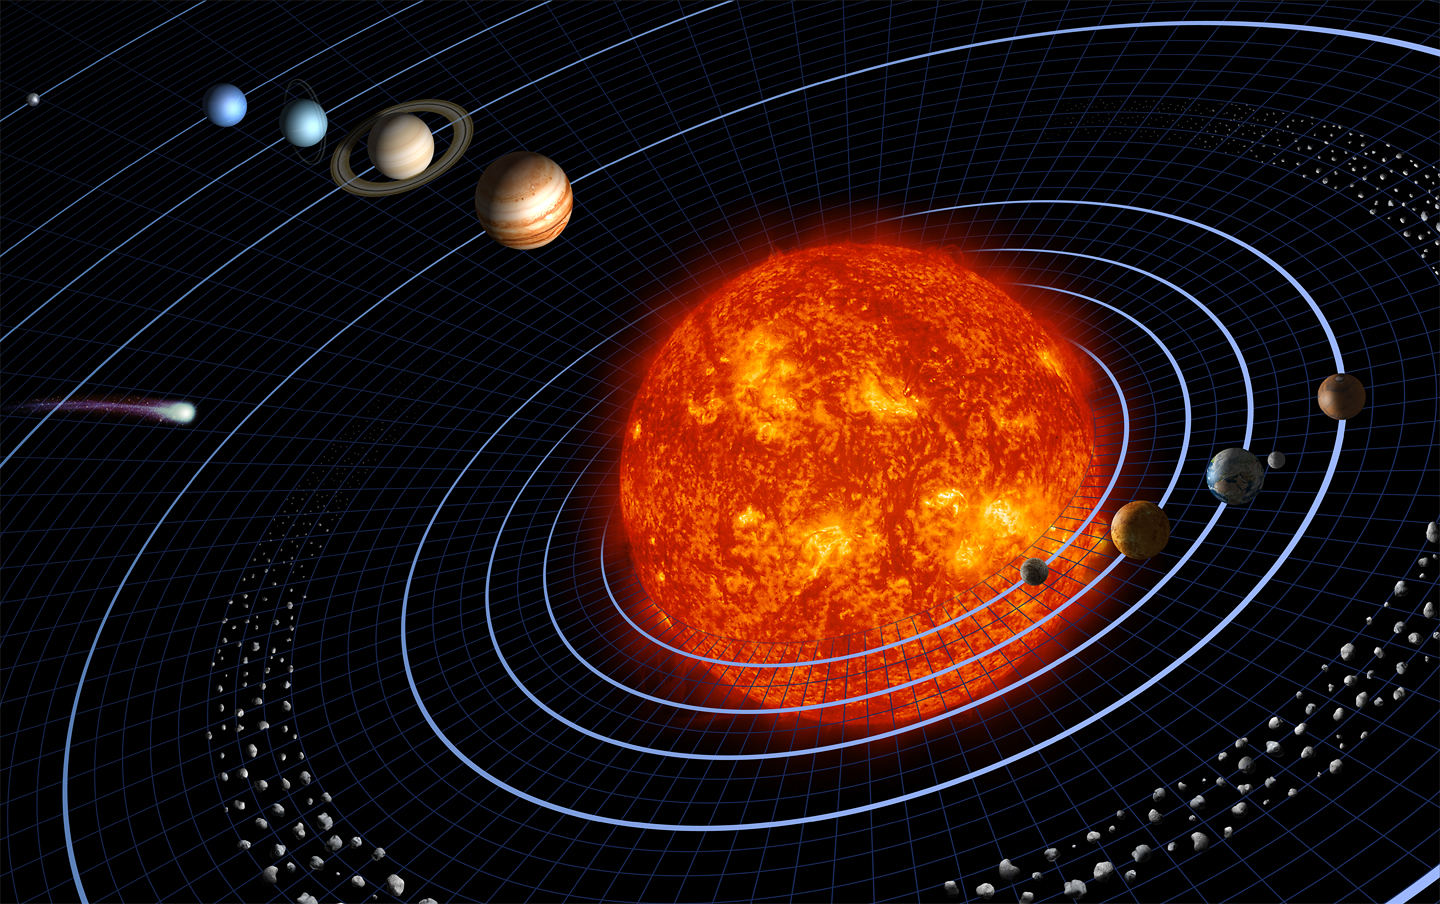
\includegraphics[draft=false,width=0.8\textwidth]{solar_system.jpg}
\end{center} \end{minipage}
\pause
\begin{minipage}{0.48\textwidth} \begin{center}
  Discretiztations of PDEs
\end{center} \end{minipage}

\pause
\vspace{2ex}

\begin{minipage}{0.48\textwidth}\begin{center}
  Granular systems

  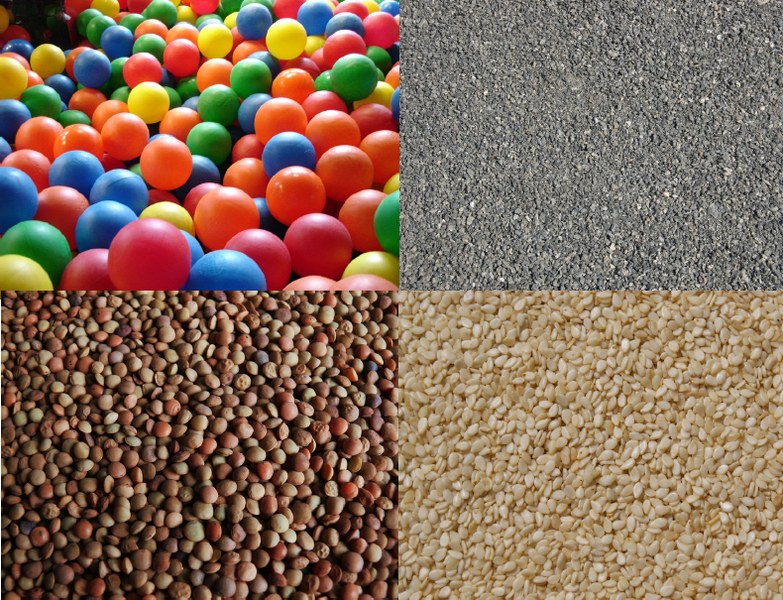
\includegraphics[draft=false,width=0.65\textwidth]{granular_system.png}
 \end{center} \end{minipage}
\pause
\begin{minipage}{0.48\textwidth}\begin{center}
  ODEs on graphs

  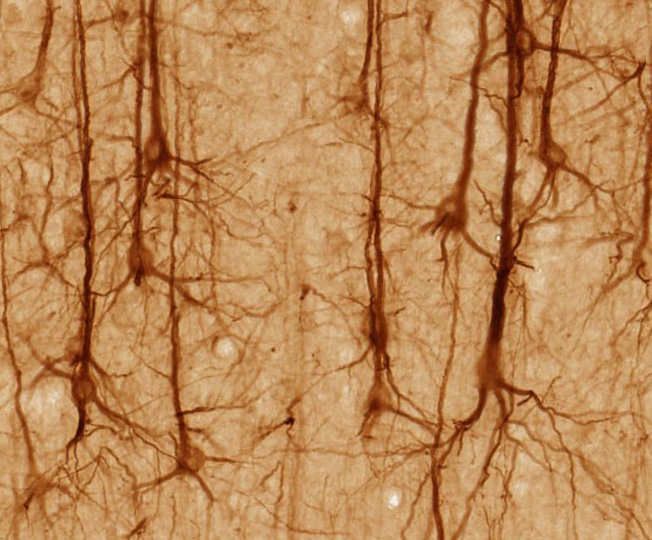
\includegraphics[draft=false,width=0.6\textwidth]{neuron.jpg}
 \end{center}\end{minipage}

 \vspace{2ex}
 \centerline{\bf High-Performance-Computing}

\end{frame}



\begin{frame}[fragile]
 \heading{Phase oscillator lattices}

 \vspace{2ex}

 \begin{columns}[T]
  \begin{column}{0.35\textwidth}
   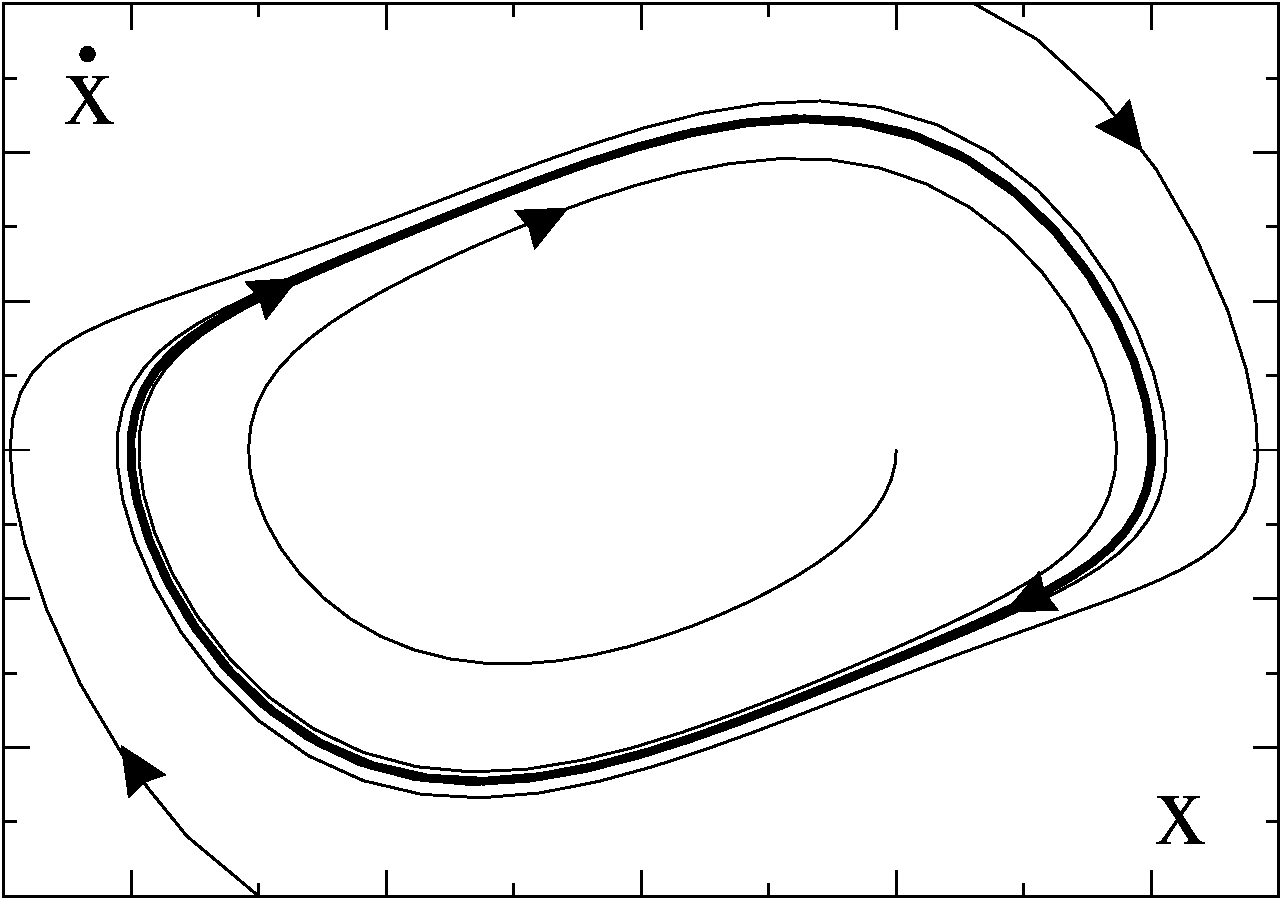
\includegraphics[draft=false,width=1.0\textwidth]{vdp.pdf}  
  \end{column}
  \begin{column}{0.63\textwidth}
 Any oscillator can be described by one variable, its phase.

 

 Trivial dynamics: $\dot{\varphi}=\omega \varphi$

 Coupled phase oscillators

 Neurosciences

 Heart dynamics

 Synchronization

 Any weakly perturbed oscillator system

 $\dot{\varphi}_k = \omega_k \varphi_k + q( \varphi_{k+1} , \varphi_k ) + q( \varphi_k , \varphi_{k-1} )$

   
  \end{column}
 \end{columns}

\end{frame}




\begin{frame}[fragile]
 
 \heading{Phase compacton lattice}

 \vspace{2ex}

 $$\dot{\varphi}_k = \cos \varphi_{k+1} - \cos \varphi_{k-1}$$

 \vspace{2ex}

 State space contains $N$ variables

 \begin{lstlisting}
typedef std::vector<double> state_type;
 \end{lstlisting}

 Animation

 Space-time plot for visualization of compactons and chaos

\end{frame}





\begin{frame}[fragile]

 \heading{Ensemble of phase oscillators}

 \vspace{2ex}

$$\dot{\varphi}_k = \omega_k + \sum\limits_l \sin( \varphi_l - \varphi_k )$$

{\bf Synchronization} -- all oscillator oscillates with the same frequency

 \vspace{2ex}

Synchronized state $\varphi_k = \omega_S t + \varphi_{0,k} $

\end{frame}



\begin{frame}[fragile]

\heading{Ensemble of phase oscillators}

\begin{lstlisting}
typedef std::vector<double> state_type;

struct ensemble
{
    state_type m_omega,m_eps;

    ensemble(size_t n,double eps)
    : m_omega(n,0.0),m_eps(eps)
    {
        create_frequencies();
    }

    void create_frequencies() { ... }

    void operator()(const state_type &x,state_type &dxdt,double t) const
    {
         ...
    }
};
\end{lstlisting}

The ODE has now many parameters, use boost::ref

Vielleicht koennen diese beiden Folien weg

\end{frame}



\begin{frame}[fragile]

\heading{Solving ODEs with CUDA using Thrust}

\vspace{4ex}
\begin{quotation}
Thrust is a parallel algorithms library which resembles the C++ Standard Template Library (STL). Thrust's high-level interface greatly enhances developer productivity while enabling performance portability between GPUs and multicore CPUs. Interoperability with established technologies (such as CUDA, TBB and OpenMP) facilitates integration with existing software. Develop high-performance applications rapidly with Thrust!
\end{quotation}

\vspace{2ex}

\centerline{
\includegraphics[draft=false,width=0.3\textwidth]{thrust_logo.png}}
 

\end{frame}


\begin{frame}[fragile]
 
\heading{Solving ODEs with CUDA using thrust}

\vspace{2ex}
Applications and use cases for GPUs:

\begin{itemize}
 \item Large systems, discretizations of PDEs, lattice systems, granular systems, etc.
 \item Parameter studies, solve many ODEs in parallel with different parameters
 \item Initial value studies, solve the same ODE with many different initial conditions in parallel
\end{itemize}


\end{frame}



\begin{frame}[fragile]
 
\heading{Lorenz system -- Parameter study}

 $$
  \dot{x} = \sigma ( y - x ) \quad \quad \dot{y} = R x - y - x z \quad \quad \dot{z} = -b z + x y
 $$

Standard parameters $\sigma=10$, $R=28$, $b=8/3$

\vspace{2ex}
Deterministic chaos -- Butterfly effect


Picture of Lorenz system

\end{frame}


\begin{frame}[fragile]
 
  \heading{Lorenz system -- Parameter study}


 $$
  \dot{x} = \sigma ( y - x ) \quad \quad \dot{y} = R x - y - x z \quad \quad \dot{z} = -b z + x y
 $$


Does one observ chaos over the whole parameter range?

\vspace{2ex}

Lyapunov exponents:
\begin{itemize}
 \item Measure of chaos
 \item Perturbations of the original system
\end{itemize}

\vspace{2ex}
Vary $R$ from $0$ to $50$ and calculate the Lyapunov exponents!

\vspace{2ex}
\centerline{\bf Use CUDA and Thrust!}

\end{frame}


\begin{frame}[fragile]

 \heading{odeint's algebras and operations}

 \vspace{2ex}

Euler method

$ x_i(t+\Delta t) = x_i(t) + \Delta t * f_i(x)$

Algebras perform the iteration over $i$ and operation the elementary addition.

Algebras and operations enter the stepper as template parameters

\begin{lstlisting}
typedef runge_kutta4<state_type,value_type,deriv_type,time_type,
    algebra,operations,resize_policy> stepper; 
\end{lstlisting}

\begin{itemize}
 \item {\tt default\_operations}
 \item {\tt range\_algebra} -- Boost.Ranges
 \item {\tt vector\_space\_algebra} -- Passes the state directly to the operations
 \item {\tt fusion\_algebra} -- For compile time sequences, like $std::tuple< double , double >$
 \item {\tt thrust\_algebra} and {\tt thrust\_algebra} -- for thrust
\end{itemize}

\end{frame}


\begin{frame}[fragile]

Thrust example for Lorenz system,

Implementation of the system function 

\end{frame}











\begin{frame}
 More advanced features, die themen können auch auf mehreren folien zusammengefasst werden
\end{frame}


\begin{frame}
 Boost::ref
\end{frame}

\begin{frame}
 boost::range
\end{frame}

\begin{frame}
 complex state types, vielleicht auch nicht
\end{frame}

\begin{frame}
 arbitrary precision types
\end{frame}

\begin{frame}
 matrices as state types
\end{frame}

\begin{frame}
 graph as state types
\end{frame}

\begin{frame}
 self expanding lattices
\end{frame}








